
\subsection{Hardware}
\label{subsec:hardware} 

This subsection will explain how the project was started, to be able to rapidly prototype the main functions to allow interacting with the electronics of the plush toy.

\subsubsection{Initial breadboard solution \& development kit selection}
\label{subsubsec:hardware/development_kit_selection} 

To quickly start prototyping the firmware of the plush toy, a breadboard solution was needed as fast as possible. To this end, several development kits have been explored.

\medskip The first breadboard solution is presented figure \ref{fig:EE_Arduino_breadboard_solution}.

\begin{figure}[H]
    \centering
    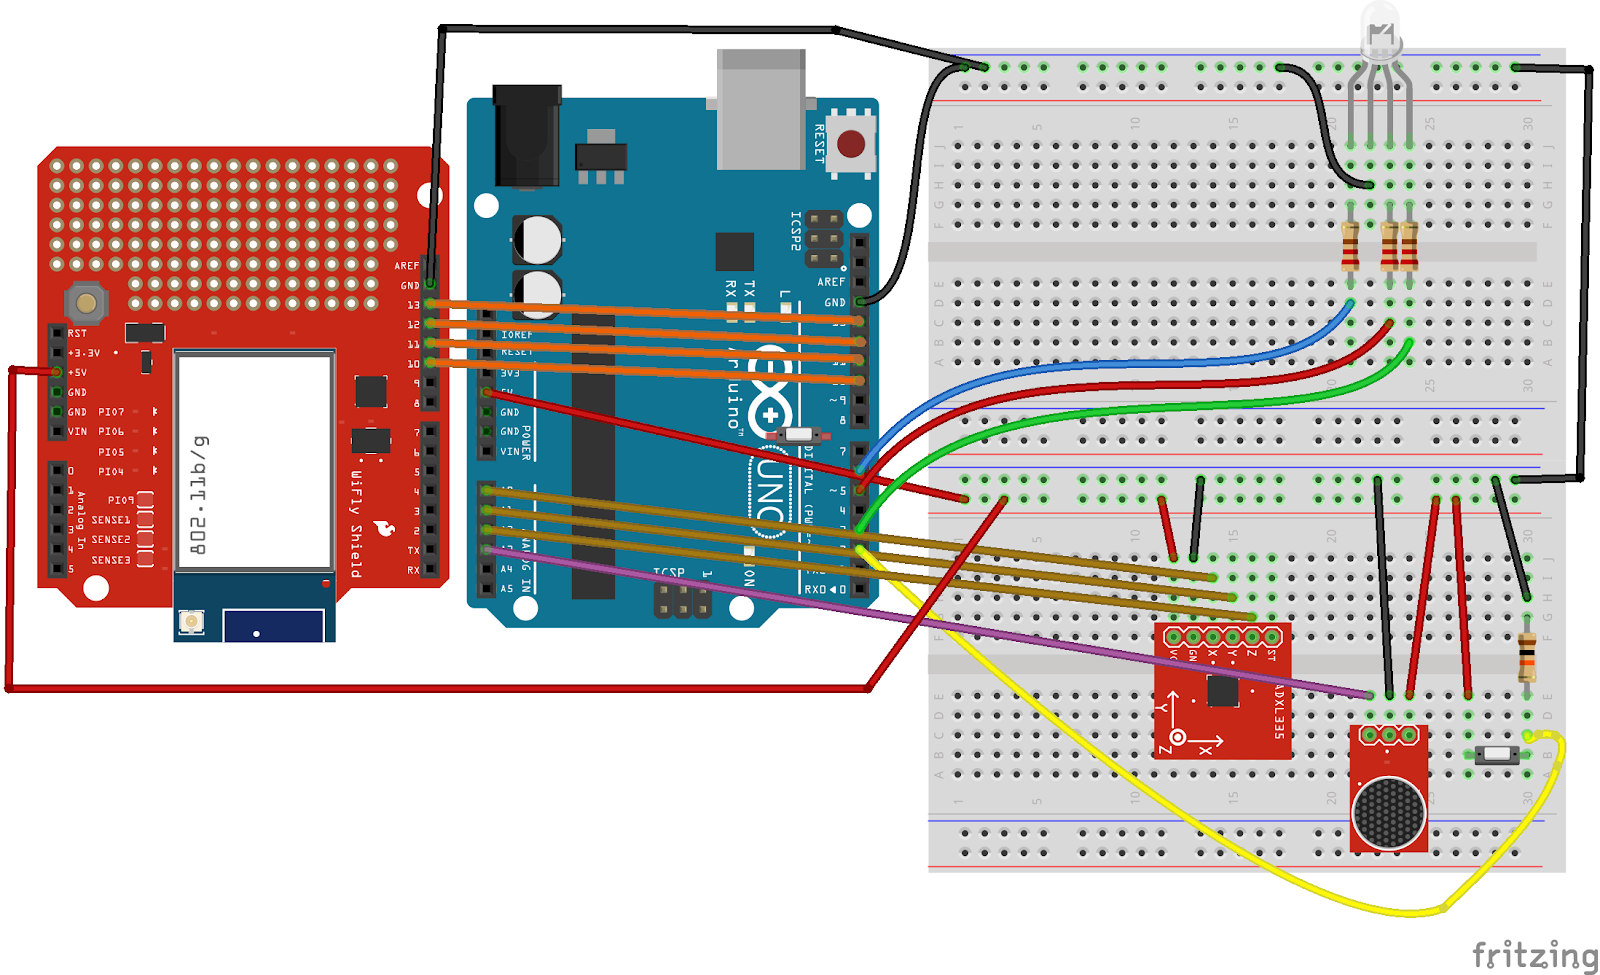
\includegraphics[width=0.5\textwidth]{images/EE_Arduino_breadboard_solution.png}
    \caption{First breadboard solution with Arduino (realized with \textit{fritzing})}
    \label{fig:EE_Arduino_breadboard_solution}
\end{figure}

This early breadboard solution was equipped of the following electronic components : 

\begin{itemize}
    \item an Arduino UNO (Rev3) - ICSP board, based on the ATmega328 microcontroller,
    \item an Arduino WiFly Shield, to equip the system with 802.11b/g wireless connection,
    \item a triple axis accelerometer breakout - ADXL335, for sensing three-dimensional accelerations,
    \item a breakout board for Electret microphone, with a 100x opamp to amplify the recorded sounds,
    \item a tri-color LED with red, green and blue inside, for the visual interaction between the plush toy and the child,
    \item and a generic pushbutton, to be able to have a tactile interaction, again between the plush toy and the child. 
\end{itemize}

At that stage of ideation, the plush toy was supposed to record the child and allow the parents or the caregivers listening to the kid. 

\medskip Figure \ref{fig:EE_Arduino_block_diagram} illustrates the block diagram related to this early breadboard solution.

\begin{figure}[H]
    \centering
    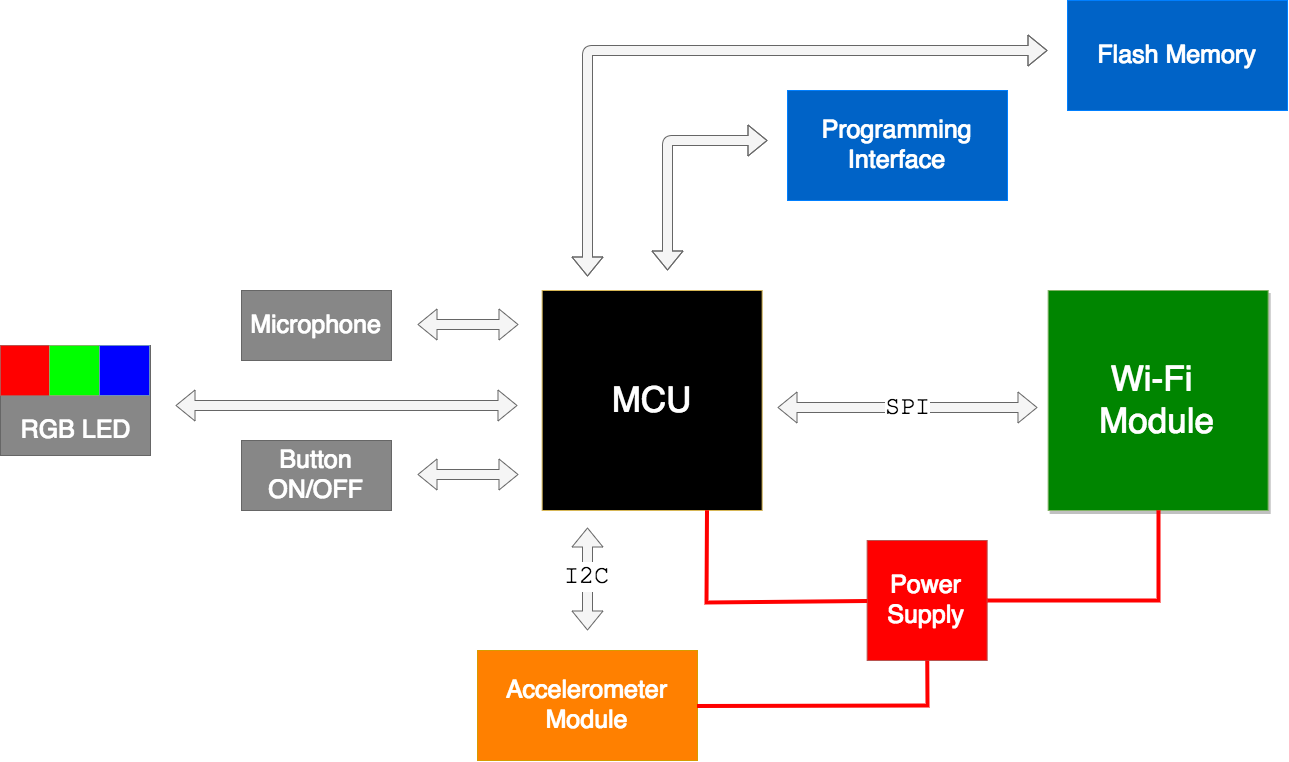
\includegraphics[width=0.6\textwidth]{images/EE_Arduino_block_diagram.png}
    \caption{First breadboard solution with Arduino}
    \label{fig:EE_Arduino_block_diagram}
\end{figure}

As it can be seen from figure \ref{fig:EE_Arduino_block_diagram}, the microcontroller would communicate with the Wi-Fi module via the SPI protocol and with the accelerometer module via I2C.There would have been a flash memory to store the voice recordings of the child. Obviously, the system would have also been equipped of a tri-color LED, a pushbutton and a microphone, as previously illustrated \ref{fig:EE_Arduino_breadboard_solution}.

\medskip After seeking for related work on toys with this recording feature, it has been understood that it was not only too invasive for the child's privacy, but also very risky on the cyber-security domain (\cite{mcreynolds2017toys}). Therefore, the recording feature has been abandoned. The electronics in care of the interaction between the plush toy and the child have also been largely enhanced, through the use of capacitive soft sensors (more details section \ref{sec:me}).

\medskip The final development kit that has been used is the ESP32-DevKitC, shown figure \ref{fig:ESP32-DevKitC}. 

\begin{figure}[H]
    \centering
    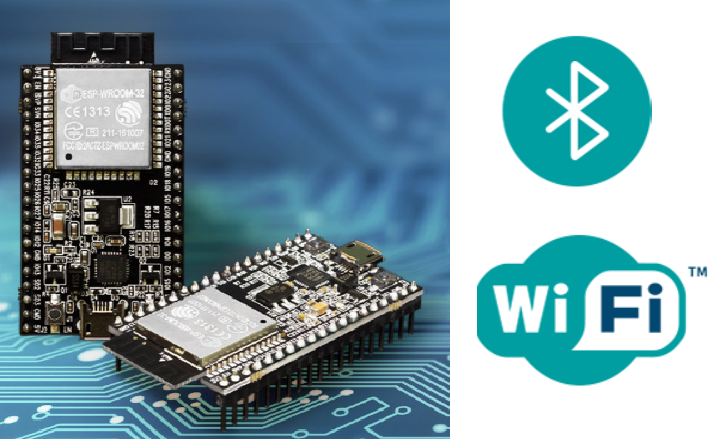
\includegraphics[width=0.6\textwidth]{images/EE_wifi_BLE.PNG}
    \caption{ESP32-DevKitC}
    \label{fig:ESP32-DevKitC}
\end{figure}




\subsubsection{ESP32 Capabilities \& final breadboard solution}
\label{subsubsec:hardware/esp32_capabilities} 

The reasons of this choice of development kit can be even more clearly seen with the following comparison.

\begin{figure}[H]
    \centering
    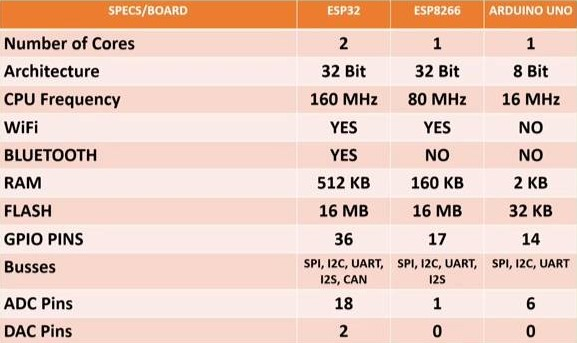
\includegraphics[width=0.6\textwidth]{images/EE_Comparaison_ESP32_ArduinoUNO.jpg}
    \caption{Comparison between ESP32, ESP8266 and Arduino UNO boards capabilities (\cite{esp32futureelectronics})}
    \label{fig:Comparison_ESP32_ArduinoUNO}
\end{figure}

\medskip Various capabilities of the ESP32-DevKitC are developed here below.

\begin{description}[align=left]
    \item[CPU architecture] The ESP32-DevKitC has a 32-bit double core CPU, one dedicated for the wireless (Wi-Fi and Bluetooth) and the other for the logic and control.
    \item[GPIO pins] There are up to 16 channels of PWM-capable pins, for dimming LEDs or controlling motors. Up to 10 channels feature capacitive touch sensors.
    \item[UART] There are two UART interfaces to load code serially, feature flow control and support IrDA (Infrared Data Association).
    \item[I2C, SPI, I2S] There are two I2C and four SPI interfaces to hook up all types of sensors and peripherals, plus two I2S interfaces for connecting digital audio devices.
    \item[Analog-to-Digital Converter (ADC)] With up to 18 channels of 12-bit signals, the ADC range can be set, in firmware, to either 0-1V, 0-1.4V, 0-2V, or 0-4V.
    \item[Digital-to-Analog Converter (DAC)] There are two 8-bit DACs to produce true analog voltages.
\end{description}

\medskip Thus, this development kit allows rapid prototyping and flexibility with its Wi-Fi and BLE (Bluetooth Low Energy) connectivity. The firmware is easy to program, thanks to its Arduino IDE (integrated development environment) compatibility and its peripherals. 

\newpage Figure \ref{fig:ESP32-DevKitC_functional_overview} shows the key components of the ESP32-DevKitC.

\begin{figure}[H]
    \centering
    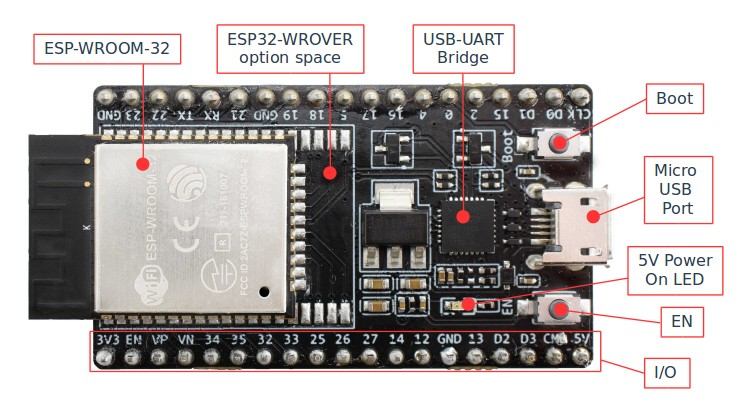
\includegraphics[width=0.6\textwidth]{images/EE_esp32-devkitc-functional-overview.jpg}
    \caption{ESP32-DevKitC functional overview (\cite{esp32gettingstartedguide})}
    \label{fig:ESP32-DevKitC_functional_overview}
\end{figure}

Its micro USB port and the boot button allow an easy connectivity to program the ESP32 microcontroller, embedded inside the ESP-WROOM-32 unit. The development kit already includes a USB-UART bridge, translating the program coming from the computer, via USB, to the microcontroller in UART protocol. The EN pushbutton "ENables" to reset the microcontroller, starting again the program from the first line of code. The ESP32-WROVER optional space has not been used, since it is a different microcontroller chip, longer than the ESP-WROOM-32. 

\medskip The large number of available input/output pins were very useful to develop our final breadboard solution, shown figure \ref{fig:ESP32_breadboard_solution}.

\begin{figure}[H]
    \centering
    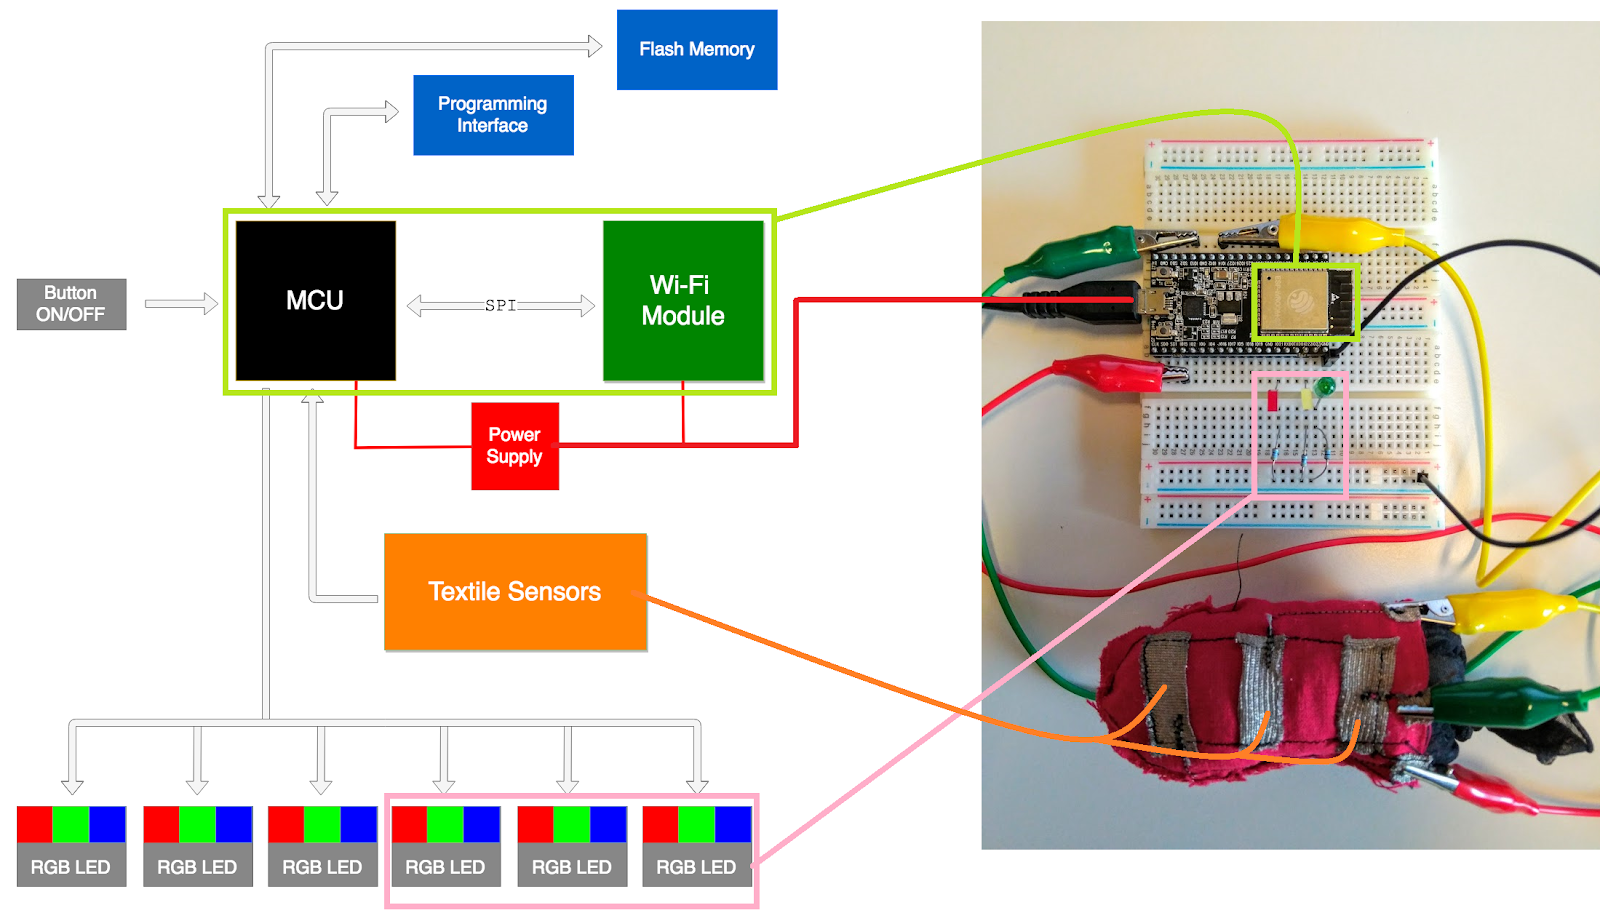
\includegraphics[width=0.6\textwidth]{images/EE_ESP32_breadboard_solution.png}
    \caption{Final breadboard solution using ESP32-DevKitC}
    \label{fig:ESP32_breadboard_solution}
\end{figure}

The main addition with the initial breadboard solution, illustrated figure \ref{fig:EE_Arduino_breadboard_solution}, is the presence of capacitive textile sensors instead of pushbuttons. This replacement definitely enhanced the user experience of the child, eventually interacting by simply touching the paws of the plush toy. At that stage of the project, the shape was not defined yet and could have represented any animal, like other mainstream teddybears.

\medskip Another replacement on the hardware side was to remove the microphone, initially supposed to record the child's voice. Instead, a miniature speaker (figure \ref{fig:MiniatureSpeaker}) has been added, to be able to play sounds for every LED that lights up. 

\begin{figure}[H]
    \centering
    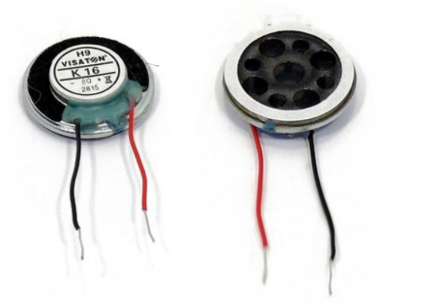
\includegraphics[width=0.3\textwidth]{images/EE_MiniatureSpeaker.PNG}
    \caption{Miniature speaker of 2 grams, 16 mm diameter and 3.5 mm depth (\cite{minispeakerspec})}
    \label{fig:MiniatureSpeaker}
\end{figure}

The tri-color LEDs that have been used for our final product are the APA102C (figure \ref{fig:APA102C}).

\begin{figure}[H]
    \centering
    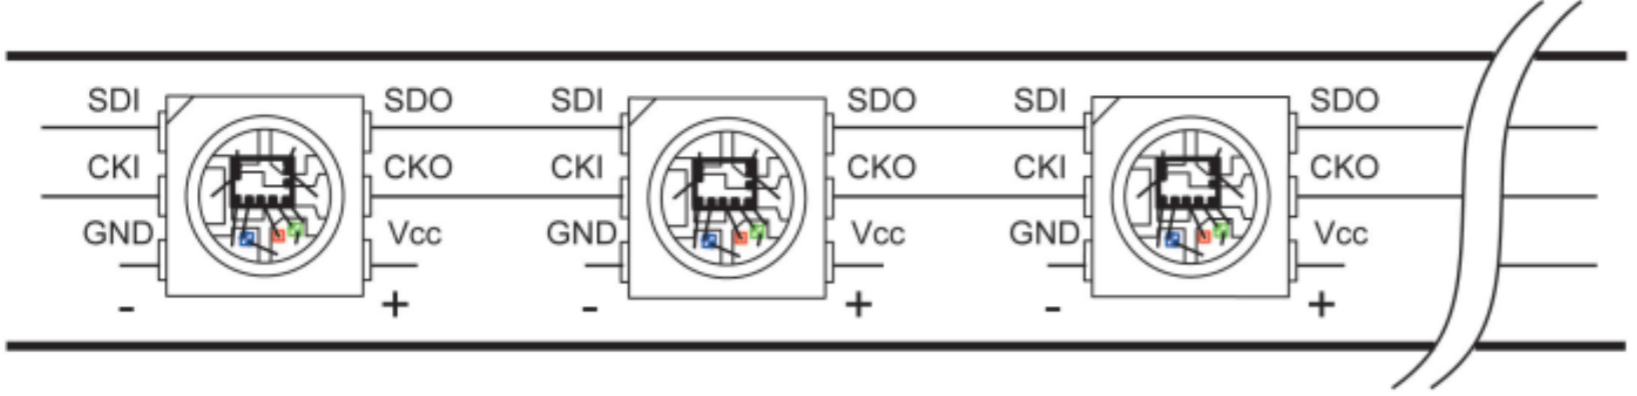
\includegraphics[width=0.6\textwidth]{images/EE_APA102C.PNG}
    \caption{LED strip of tri-color RGB LEDs APA102C (\cite{ledstripspec})}
    \label{fig:APA102C}
\end{figure}

\noindent SDI/SDO : Serial Data Input/Output \newline CKI/CKO : Clock Input/Output \newline GND : Ground -- VCC : 5V

\medskip As illustrated above, the main advantage of these LEDs is their capability of commanding a strip of N LEDs with only 2 command signals (SDI and CKI). More information on their functioning will be provided subsection \ref{subsec:fw/Functions/LEDs}.


\newpage
\subsubsection{Electronic characteristics}
\label{subsubsec:hardware/electronic_characteristics} 

Now will be described the different power modes, available on the ESP32 microcontroller, allowing a reduction of power consumption depending on the state of the ESP32 microprocessor.

\begin{figure}[H]
    \centering
    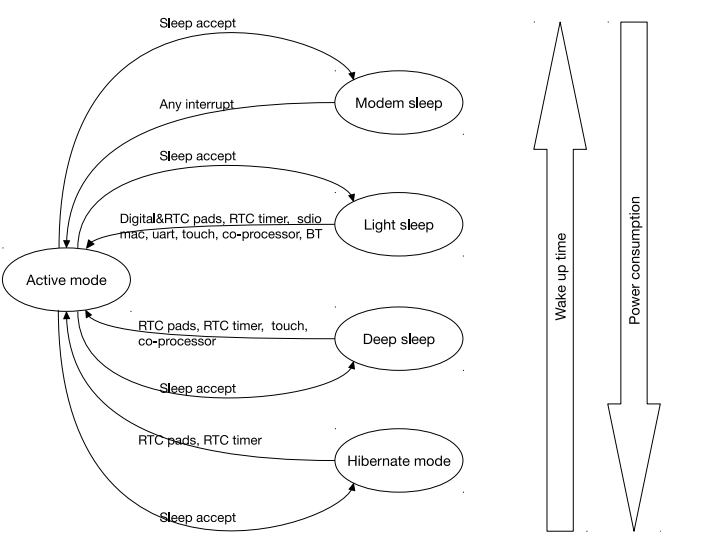
\includegraphics[width=0.6\textwidth]{images/EE_PowerModes.PNG}
    \caption{Power modes of the ESP32 microprocessor (\cite{esp32techrefmanual})}
    \label{fig:power_modes}
\end{figure}

\begin{figure}[H]
    \centering
    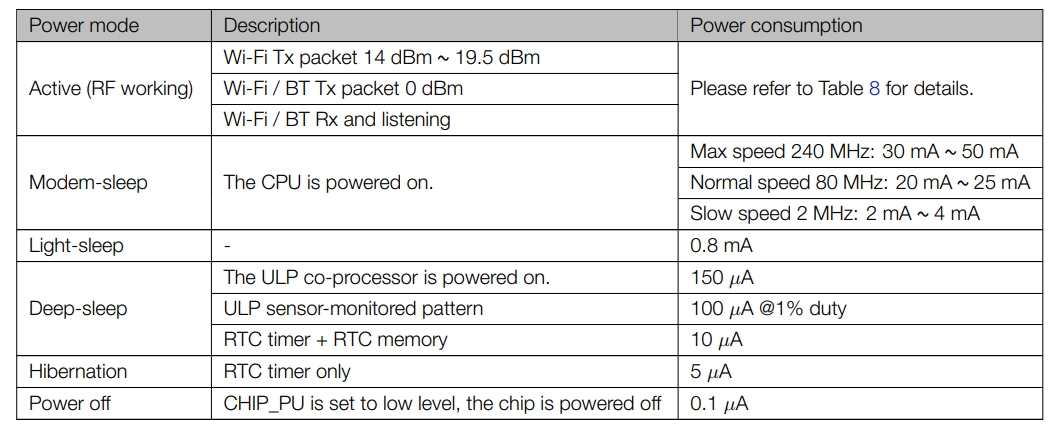
\includegraphics[width=0.6\textwidth]{images/EE_PowerConsumption.PNG}
    \caption{Power consumption by power modes (\cite{esp32datasheet})}
    \label{fig:power_consumption}
\end{figure}

\begin{figure}[H]
    \centering
    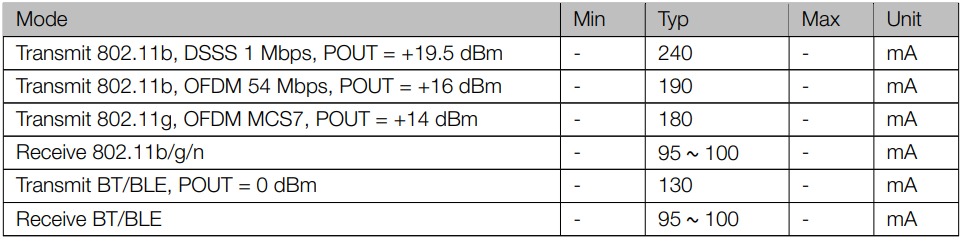
\includegraphics[width=0.6\textwidth]{images/EE_PowerConsumption2.PNG}
    \caption{Radio frequency power consumption specifications  (\cite{esp32datasheet})}
    \label{fig:power_consumption2}
\end{figure}

\newpage From figures \ref{fig:power_modes}, \ref{fig:power_consumption} and \ref{fig:power_consumption2} have been extracted the values of power consumption for the estimation of the battery life.

\begin{itemize}
    \item Powering 9 LEDs APA102C, drawing 20 mA of constant current each, requires to output $I_{LEDs} = 9*20 = 180$ mA (\cite{ledstripspec}).
    \item The maximum power of the miniature speaker is 1 W, which corresponds to $I_{speaker} = 200$ mA of current consumption for a voltage output of 5 V.
    \item During Wi-Fi transmissions, the microcontroller requires from 180 to 240 mA. Considering the largest possible current consumption : $I_{WiFi} = 240$ mA.
    \item When the ESP32 enter the \textit{deep-sleep} mode, the microcontroller only requires \\$I_{DeepSleep} = 0.15$ mA.
\end{itemize}

\medskip From these values, the maximal and minimal current consumption values are:

\begin{gather}
    I_{max} = I_{LEDs} + I_{speaker} + I_{WiFi} = 180 + 200 + 240 = 620 \text{ mA} \\ \notag\\
    I_{min} = I_{DeepSleep} = 0.15 \text{ mA} 
\end{gather}

\medskip Using an \textit{Energizer} EN22 non-rechargeable battery (figure \ref{fig:recharg_battery}), with a 9V nominal voltage and a battery capacity of $Cap = 625$ mAh, the maximal and minimal battery lifetime have been estimated as follows.

\begin{gather}
    T_{max} = \frac{Cap}{I_{min}} = \frac{625}{0.15} = 4166.67 \textit{ h} = 173.6 \text{ days} = 5.8 \text{ months}\\ \notag \\
    T_{min} = \frac{Cap}{I_{max}} = \frac{625}{620} = 1.0 \textit{ h}
\end{gather}

These numbers need to be considered as a range of battery lifetime. The LEDs have been considered all simultaneously lighted on with maximal brightness and the speaker on maximal power. Also, the Wi-Fi has been considered continuously transmitting.

\medskip In the prototyping phase, an \textit{Energizer} NH22-175 rechargeable battery will be preferred, to ease the testing procedure. With a capacity of 175 mAh, $T_{max} = 6.9$ weeks and $T_{min} = 16.9$ min.

\begin{figure}[H]
    \centering
    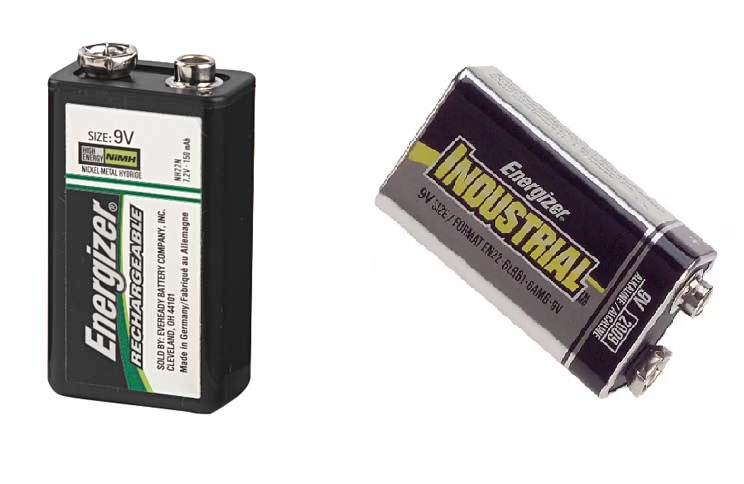
\includegraphics[width=0.30\textwidth]{images/EE_Battery.JPG}
    \caption{NH22-175 rechargeable battery (\cite{batterydatasheet}) on the left and EN22 non-rechargeable battery (\cite{battery2datasheet}) on the right}
    \label{fig:recharg_battery}
\end{figure}


